\section{Geometric Analyses} \label{sec:geometric}

In this section, we consider the geometry that tag matching metrics construct over bitstring tag space.


Geometric constraints of tag matching metrics may affect the patterns of tag connectivity that tend to, or even can, arise under a
In a constrained, it is possible for there to be two queries such that no operand can match both queries well.
Likewise, it is possible for there to be two queries such that an operand must match both queries well.

Structure might prove useful to facilitate modularity, where subsets of tag space tend to have associated functionality.
However, it may also constrain the ease (or possibility) at which adaptive variation can be generated.

To get at these questions, we compare distributions of two statistics measuring constraint across our five tag-matching metrics.
\begin{figure}
\begin{center}

\begin{minipage}{0.45\linewidth}
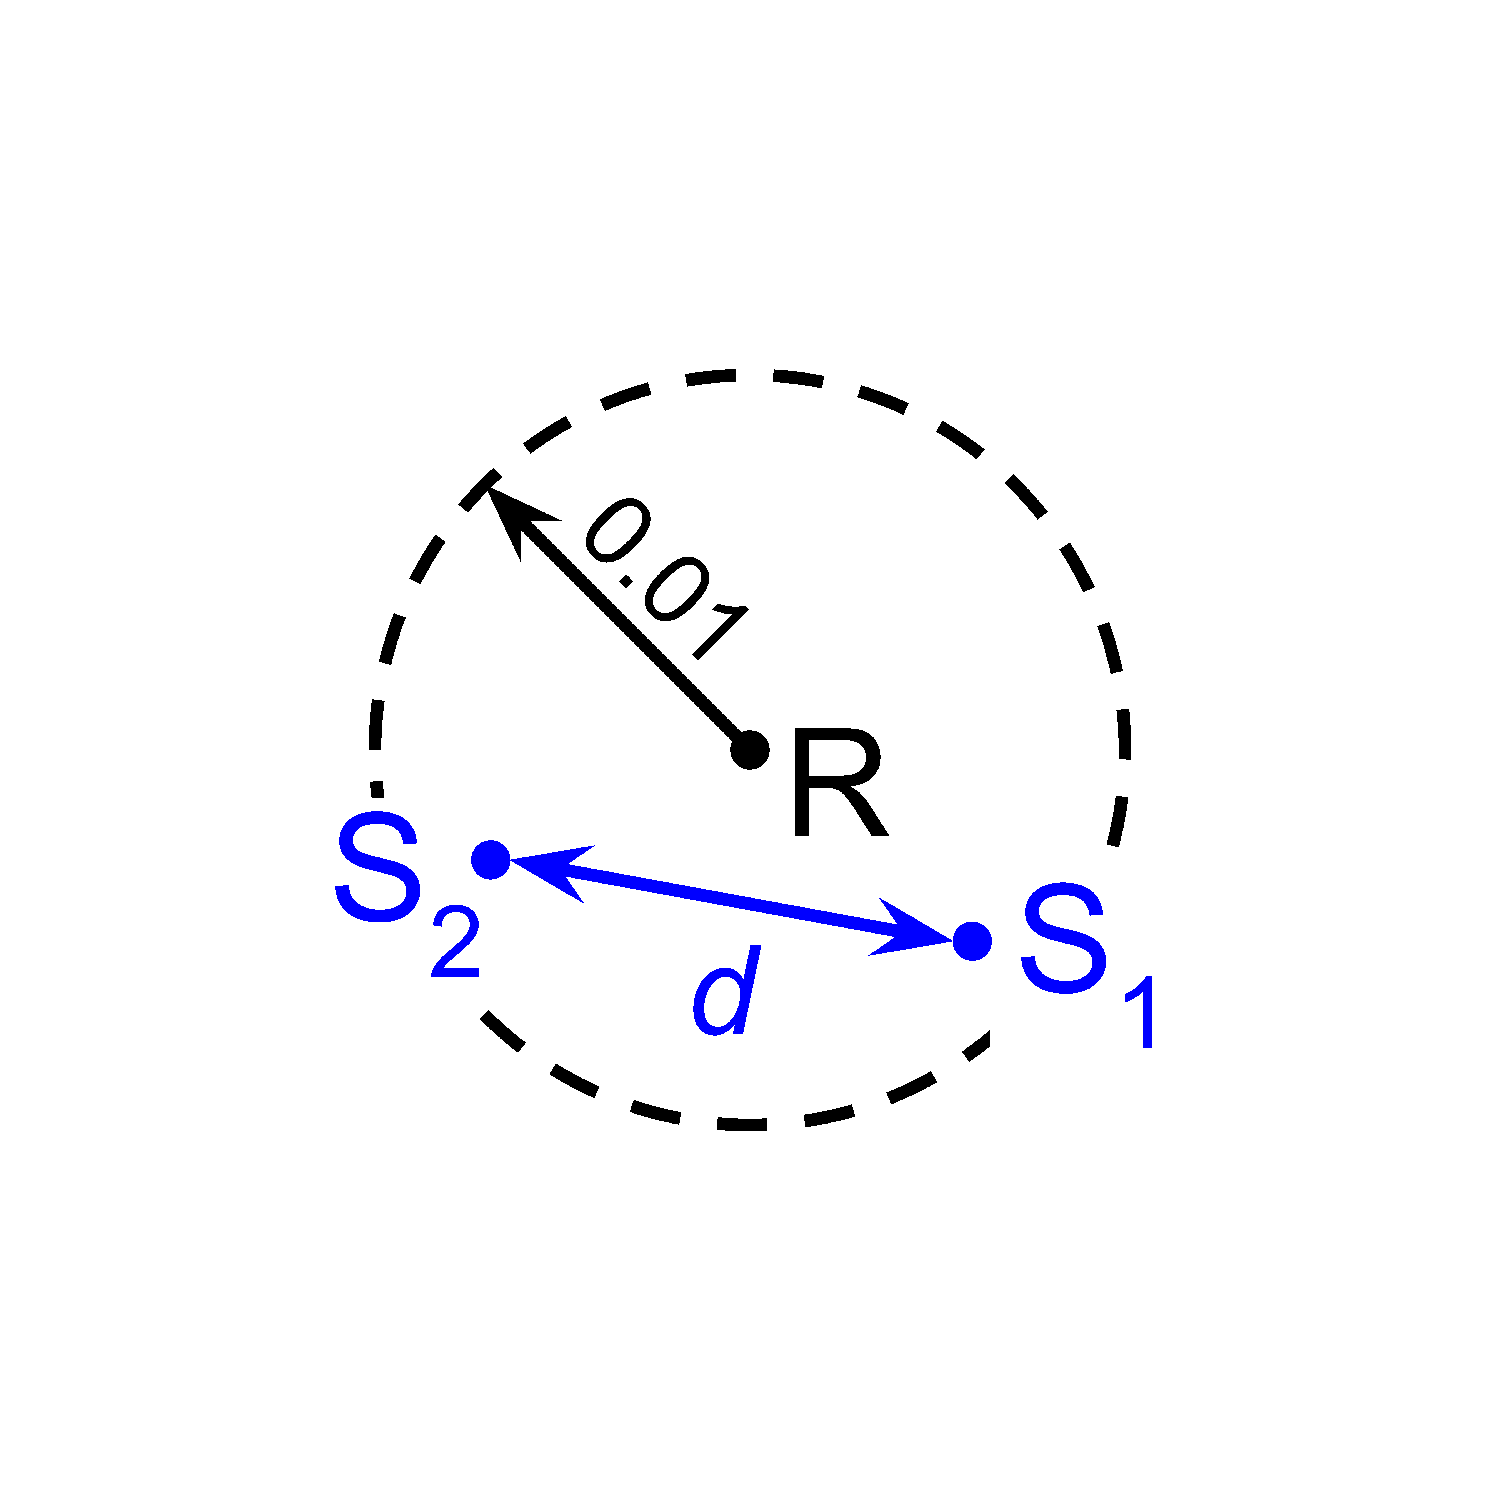
\includegraphics[width=\linewidth]{dimensionality-statistic}
\end{minipage}
\begin{minipage}{0.45\linewidth}
\caption{
The sampling process used to calculate similarity constraint for each metric.
}
\label{fig:dimensionality_measure}
\end{minipage}
\end{center}
\end{figure}


The first statistic we calculate is similarity constraint.
This statistic quantifies the question, "If two tags both match closely to a third tag, will they necessarily match closely with each other?"
To compute this statistic, we randomly sampled 5000 target tags.
Then, for each target tag we randomly sampled tags until we found two secondarily-sampled tags that were within a 0.01 match distance radius to the target.
Finally, we computed the match distance between the pair of seconarily-sampled tags.
Figure \ref{fig:dimensionality_measure}(a) summarizes this process.

The second statistic we calculate is dissimilarity constraint.
This statistic quantifies the question, "If a tag matches a second tag closely and a third tag poorly, will the second and third tag tend to match poorly?"
To compute this statistic, we randomly sampled 5000 target tags.
Then, for each target tag we randomly sampled tags until we found a secondarily-sampled tag that was within a 0.01 match distance radius of the target and a secondarily-sampled tag that was outside a 0.99 match distance radius of the target.
Finally, we computed the match distance between the pair of secondarily-sampled tags.
Figure \ref{fig:dimensionality_measure}(a) summarizes this process.

\subsection{Similarity Constraint}

\begin{figure*}
\begin{center}

\begin{minipage}{0.15\linewidth}
\begin{subfigure}[b]{\linewidth}
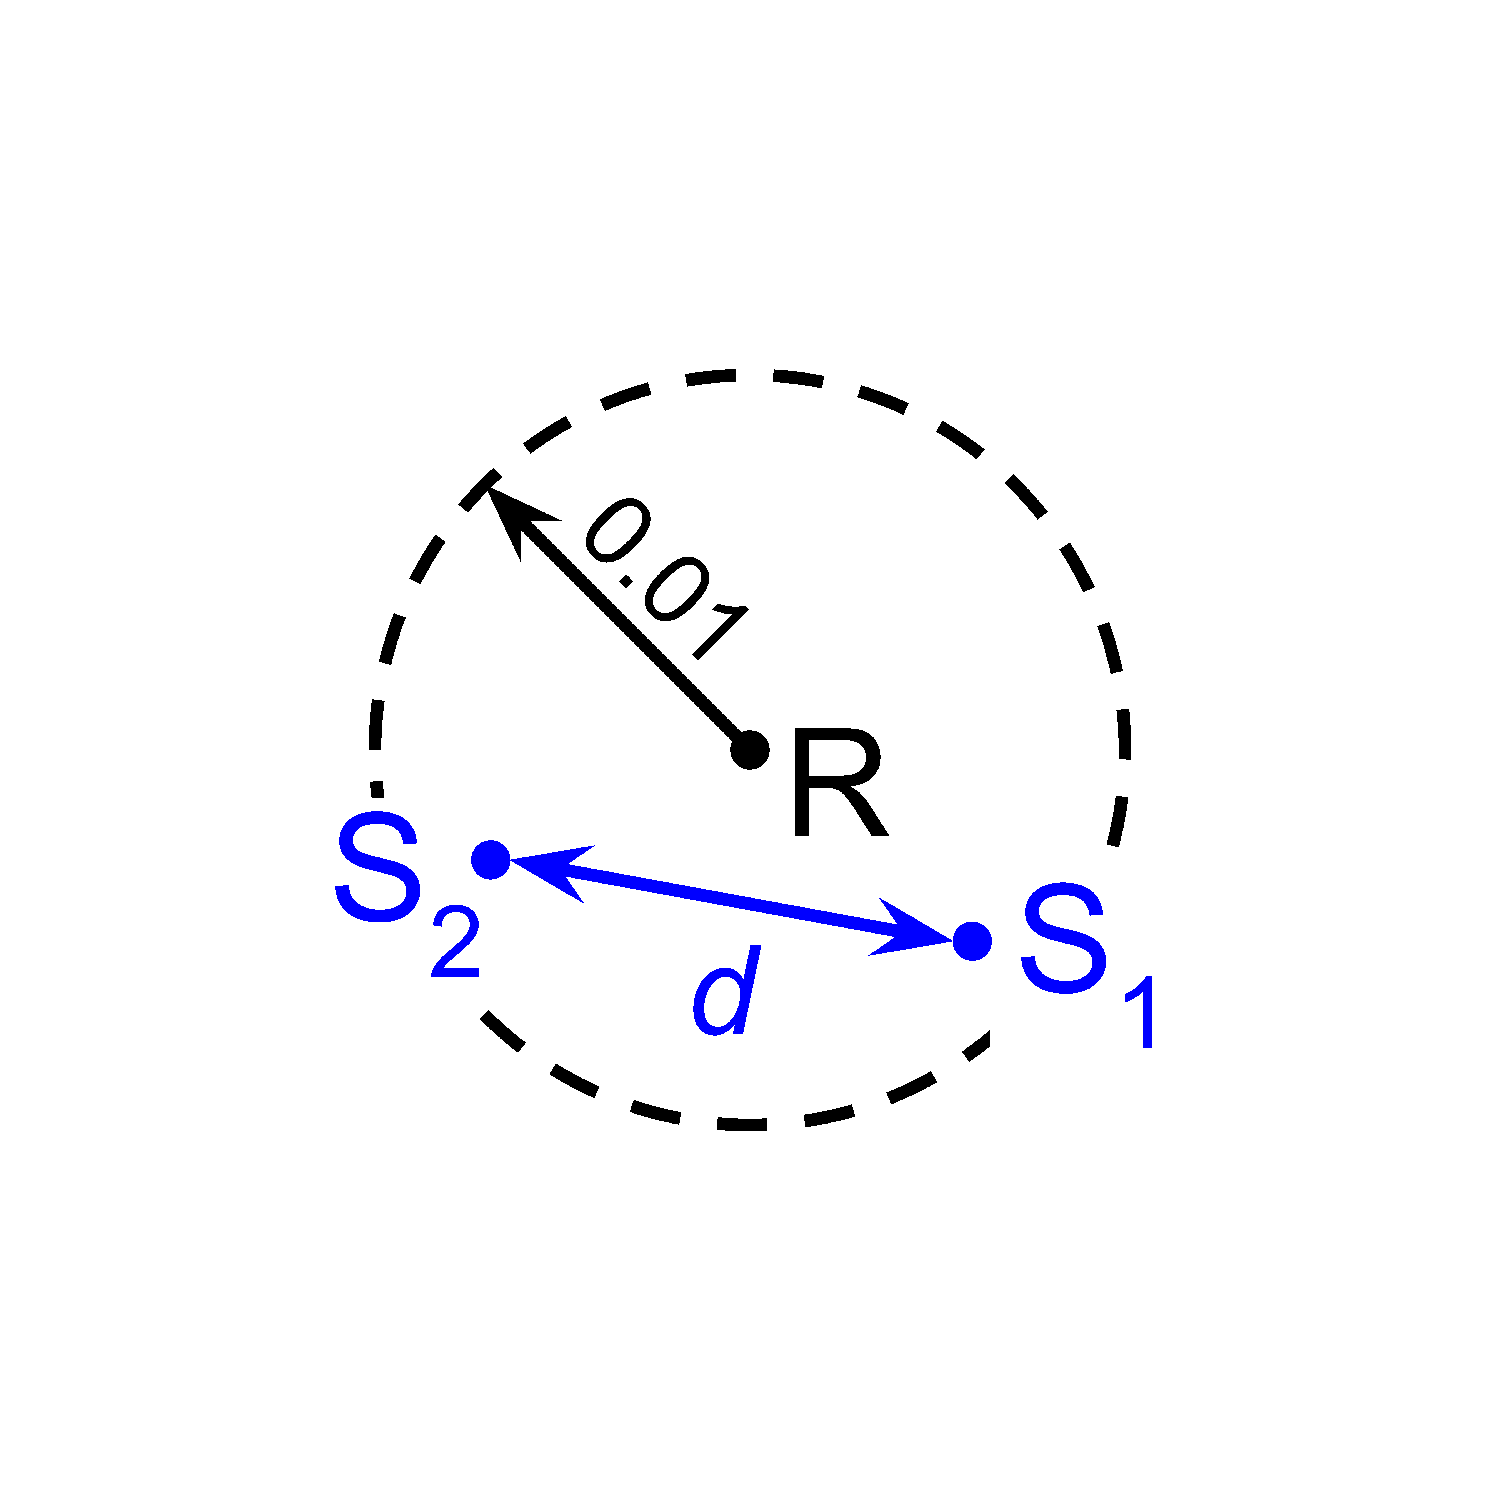
\includegraphics[width=\linewidth]{dimensionality-statistic}
\caption{
The sampling process used to calculate similarity constraint for each metric.
}
\end{subfigure}
\end{minipage}%
\begin{minipage}{0.35\textwidth}
\begin{subfigure}[b]{\linewidth}
\centering
\includegraphics[width=\linewidth]{sphere/bitweight=0dot5+seed=1+title=dimensionality_barplot+_data_hathash_hash=c0f6c5cf854ff253+_script_fullcat_hash=03ce1e318a24a109+ext=}
\caption{
Mean statistic values for each metric.
Error bars represent 95\% confidence intervals.
}
\label{fig:sphere_distnplot}
\end{subfigure}
\end{minipage}%
\begin{minipage}{0.5\linewidth}
\begin{subfigure}[b]{\linewidth}
\centering
\includegraphics[width=\linewidth]{sphere/bitweight=0dot5+seed=1+title=dimensionality_distnplot+_data_hathash_hash=c0f6c5cf854ff253+_script_fullcat_hash=03ce1e318a24a109+ext=}
\caption{
Statistic distribution, where each horizontal bar sliver represents one independent observation.
}
\label{fig:sphere_barplot}
\end{subfigure}
\end{minipage}

\caption{
Dimensionality statistic measured as distances between two tags sampled from within 0.01 match distance of a third tag.
}
\label{fig:sphere}

\end{center}
\end{figure*}


In a euclidean space, the similarity constraint metric would correspond to the average distance between points uniformly sampled from inside a ball (e.g., in two dimensions a circle, in three dimensions a sphere, etc.).
Average distance between such points increases with dimensionality.
For reference, in a one dimensional Euclidean space similarity constraint would measure approximately 0.0067.
In a two dimensional Euclidean space, it would measure approximately  0.0091.
In 32 dimensions, it would measure 0.0137 \citep{dunbar1997average}.

Figure \ref{fig:sphere_barplot} provides our estimate of the similarity constraint statistic for each metric, with error bars representing a 95\% confidence interval.
Figure \ref{fig:sphere_distnplot} shows the distribution of the similarity constraint statistic value among the 5000 replicate samples in greater detail.

For the bidirectional integer metric, we measured the similarity constraint statistic as 0.0068.
This falls in line with expectation: this metric is essentially identical to a one-dimensional Euclidean space.
As shown in Figure \ref{fig:sphere_distnplot}, the secondarily-sampled match distances are all bounded by the diameter of 0.02.
This metric not only exhibits tight similarity constraint in the mean case, but also permits no outliers to the similarity constraint.

The unidirectional integer metric exhibits much looser similarity constraint in the mean case.
We estimated this value as 0.5092.
However, this looser similarity constraint appears to be an artifiact of averaging between two very tight constraints: a tight constraint to 0 in one case and a tight constraint to 1 in the other.
In Figure \ref{fig:sphere_distnplot}, you can clearly see that all sampled cases fall under one of these umbrellas.
This phenomenon results from the asymmetrical definition of the metric.
If you sample pairs of similar values, half will be in ascending order (resulting in a match distance close to 0) and half will be in descending order, (resulting in a wraparound search and a match distance close to 1).
Averaging these outcomes out yields the observed mean value of 0.5.
The integer metric appears to allow for closely related tags to either very strongly match or very weakly match, but permits no intermediate outcomes.

The hamming metric exhibits a broader range of sampled similarity constraint values than the integer metrics.
We estimated mean similarity constraint as 0.1627, looser than the bidirectional integer metric.
As shown in Figure \ref{fig:sphere_distnplot}, many secondarily-sampled tag pairs are biased towards low match distances.
However, secondarily-sampled tag pairs that break this low match distance constraint are also not uncommon.
Among our 5,000 trials, we observed distances between secondarily-sampled tags as high as 0.7499.

Why is our estimate of the hamming metric similarity constraint statistic so much higher than expected in a 32-dimensional Euclidean space?
This phenomenon appears to be due to the normalization process we applied to map raw match distances to a uniform distribution.
We also calculated this statistic for the raw hamming metric without normalization.
For practical reasons, we increased the radius of our sampling sphere to 0.25.
(Only the exact target 32-bit tag satisfies within-sphere constraint with a sampling radius of 0.01.)
In 32-dimensional euclidean space with a sampling radius of 0.25, the expected distance between sampled points is 0.3415.
Our estimate of the raw hamming metric's similarity constraint statistic falls nearly in line with expectation at 0.3312.

The streak metric exhibited the next-loosest similarity constraint statistic with a mean value sampled at 0.2813.
For this metric, we observed distances between secondarily-sampled tags as high as 0.9993.
The streak metric retains some geometric constraint in the mean case, but outliers that strongly break similarity constraint are also not uncommon.

Like the integer metric, the hash metric also exhibits looser similarity constraint in the mean case.
We estimated this value as 0.5083 for the hash metric.
However, unlike the integer metric, intermediate secondarily-sampled match distances are also are possible.
In fact, secondarily-sampled match distances are uniformly distributed.
This is exactly as we would expect:
given any particular set of operands, a well-behaved hash function should yield a uniform distribution of hash results.
The hash metric exhibits no geometric structure and total geometric flexibility.

\begin{figure}[!htbp]

\begin{center}
\begin{subfigure}[b]{\linewidth}
\begin{minipage}{0.5\linewidth}

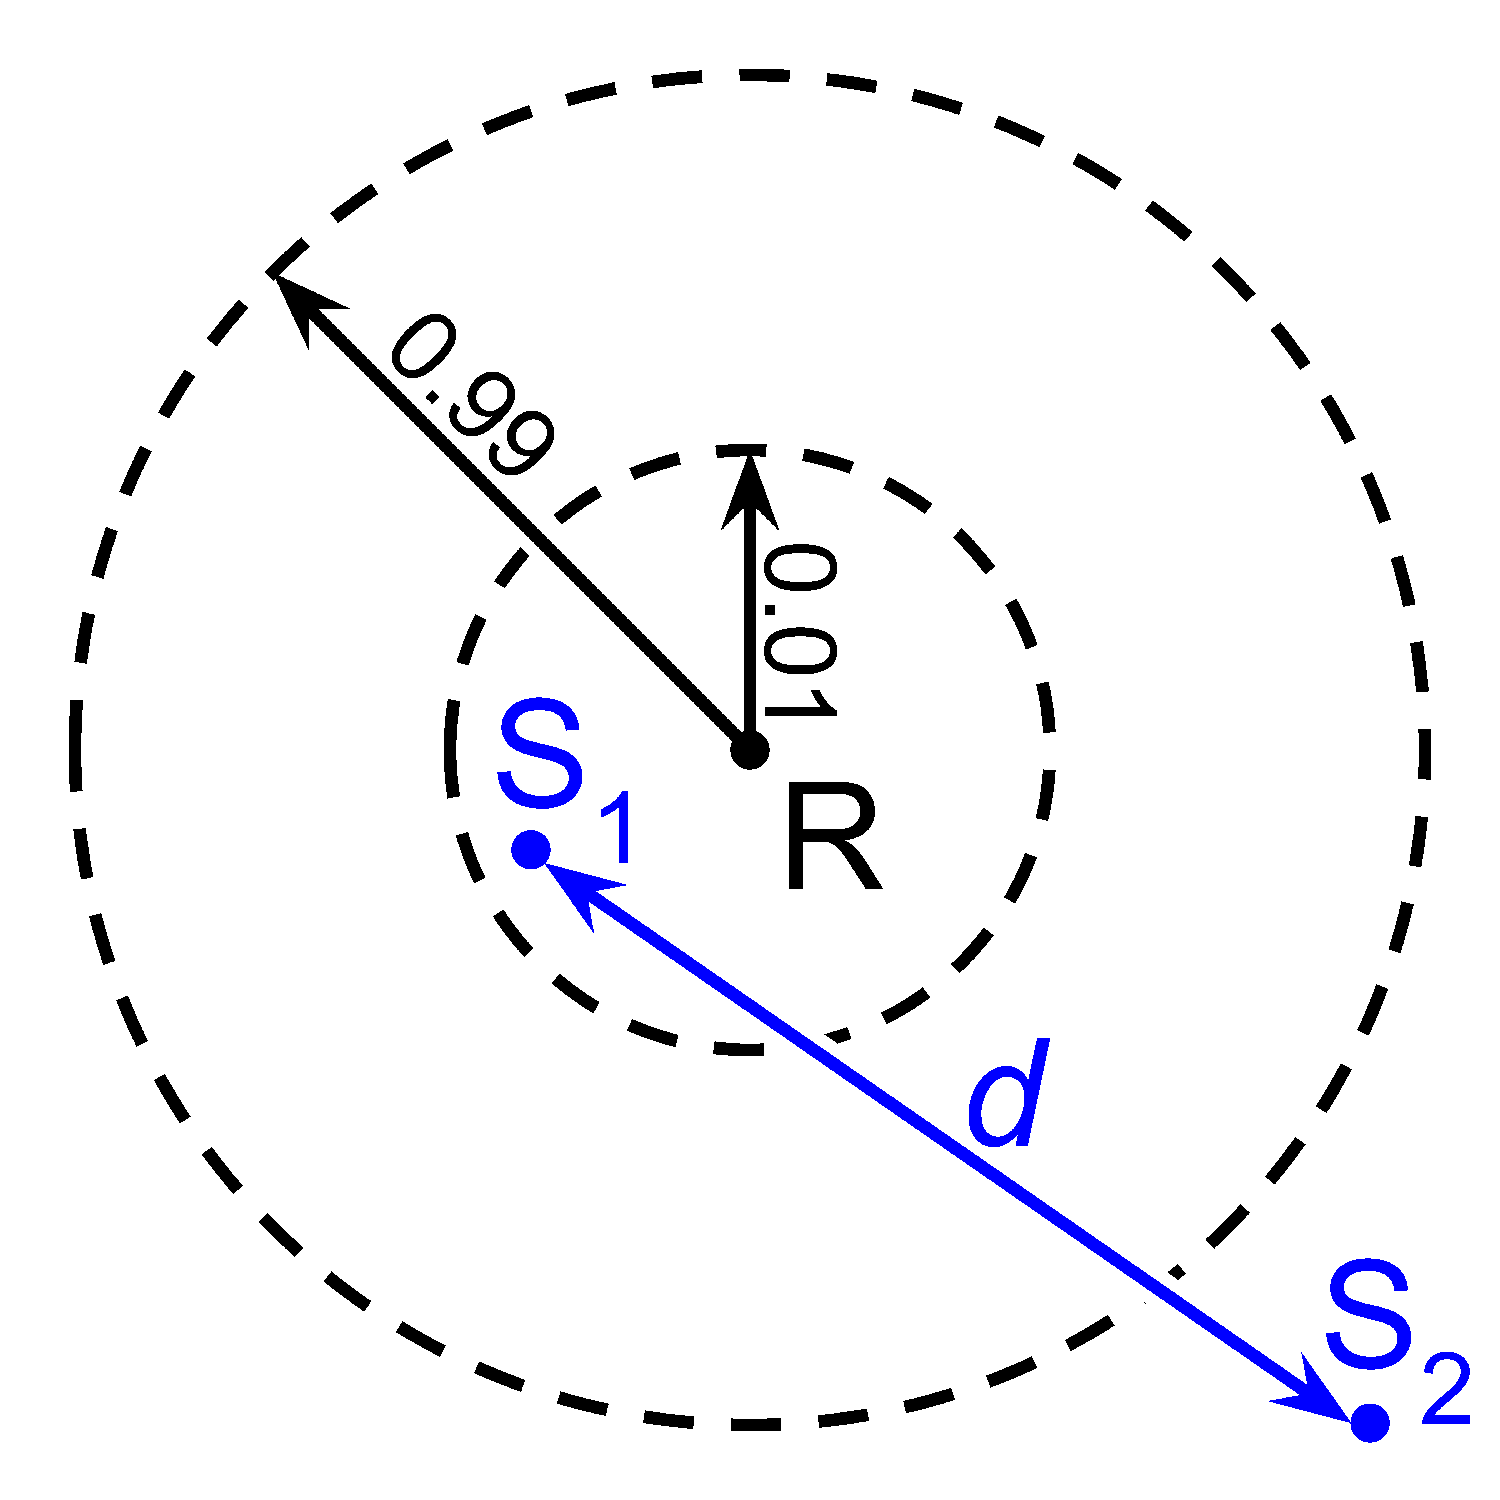
\includegraphics[width=0.75\linewidth]{img/elasticity-statistic}

\end{minipage}
\begin{minipage}{0.5\linewidth}
\caption{
Sampling process used to measure dissimilarity constraint.
First, a target tag $R$ was randomly sampled.
Then, tags were randomly drawn until a tag $S_1$ with distance to $R$ less than 0.01 was obtained.
Next, tags were randomly drawn until a tag $S_1$ with distance to $R$ more than 0.99 was obtained.
Finally, dissimilarity constraint was measured as the distance $d$ between $S_1$ and $S_2$.
}
\label{fig:dissimilarity_statistic}
\end{minipage}

\end{subfigure}

\begin{subfigure}[b]{\linewidth}
\begin{minipage}{0.6\linewidth}
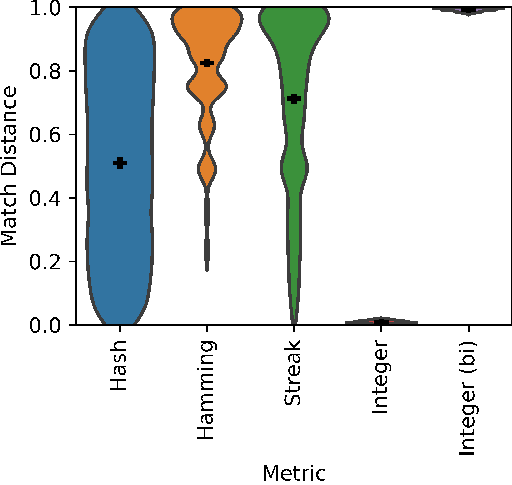
\includegraphics[width=\linewidth]{img/sphere_reverse/bitweight=0dot5+seed=1+title=dimensionality_violinplot+_data_hathash_hash=93f97a11cb443d35+_script_fullcat_hash=d1692569f79e33f8+ext=}
\end{minipage}
\begin{minipage}{0.35\linewidth}
\caption{
Mean dissimilarity constraint values for each metric.
Horizontal ticks represent means.
Error bars represent 95\% confidence intervals.
Violin plots show kernel density estimates for distribution of dissimilarity constrant.
}
\label{fig:sphere_reverse_distnplot}
\end{minipage}
\end{subfigure}
\begin{subfigure}[b]{\columnwidth}
\centering
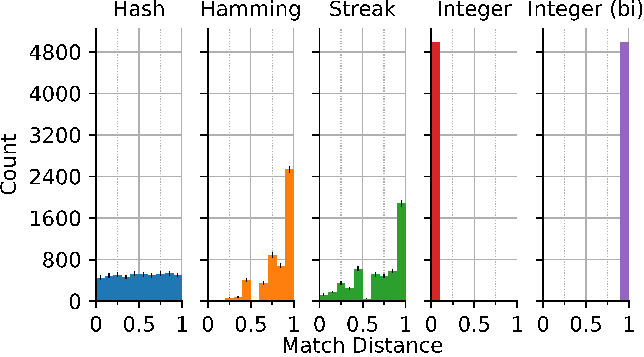
\includegraphics[width=\columnwidth]{img/sphere_reverse/bitweight=0dot5+seed=1+title=dimensionality_distnplot+viz=hist+_data_hathash_hash=93f97a11cb443d35+_script_fullcat_hash=cda229fb13f5a152+ext=}
\caption{
Frequency of sampled dissimilarity constraint values in each match distance decile.
Error bars are 95\% confidence intervals calculated using the Wilson score method with continuity correction \citep{newcombe1998two}.
}
\label{fig:sphere_reverse_barplot}
\end{subfigure}

\caption{
Dissimilarity constraint of tag-matching metrics.
Figure \ref{fig:dissimilarity_statistic} summarizes the sampling process used to measure similarity constraint.
Figures \ref{fig:sphere_reverse_barplot} and \ref{fig:sphere_reverse_distnplot} compare distributions of similarity constraint across metrics.
Supplementary Figure \ref{fig:sphere_reverse_supp} visualizes the cumulative distribution of all sampled dissimilarity constraint values for each metric.
}
\label{fig:sphere_reverse}

\end{center}
\end{figure}


We tested the elasticity of the tag-matching metrics using a similar measure.
To gain a sense of the dimensionality (in a loose sense) of the different tag-matching metrics, we sampled the distribution of distances between a tag sampled from within a 0.01 match distance radius of an arbitrary target and a tag sampled from outside a 0.99 match distance radius of the arbitrary target.
We used 5000 samples.
Figure \ref{fig:dimensionality_measure}b provides a cartoon summary of this process.

We found that the bidirectional integer metric was highly inelastic: the smallest distance between the sampled tags was 0.980201.
The mean distance between sampled tags was 0.9932740098.
The Spector integer metric exhibited similarly uniform outcomes, except the distribution was strongly pegged to 0 because of the metric's asymmetry.
The mean statistic was 0.00998706165234.

The hamming metric exhibited greater elasticity: we observed distances between the sampled tags as low as 0.235526.
The mean distance between sampled tags was 0.8248383674.

The streak metric exhibited the greatest elasticity: we observed distances between the sampled tags as low as 0.00019998.
With this metric, a tag can have a strong attractive interaction with a second tag that a third tag it interacts attractively strongly with has a strong repulsive attraction with.
The mean distance between sampled tags was 0.7126656857120001.

The hash metric exhibited the same well-behaved uniform distribution as before, with a mean distance of 0.5102822773801999.

